\documentclass[aspectratio=1610,18pt]{ctexbeamer}
\usetheme{Madrid}
% \usefonttheme{professionalfonts}
\usefonttheme{structurebold}
\usecolortheme{rose}
\setbeamerfont{title}{size=\LARGE, series=\bfseries}
\setbeamertemplate{footline}[frame number]



\usepackage{amsmath}
\usepackage{amssymb}
\usepackage{listings}
\usepackage{booktabs}
\usepackage{multirow}
\usepackage{multirow}
\usepackage{lmodern}
\usepackage{xcolor}
\usepackage{float}
\lstset{
  language=Python,  %代码语言使用的是matlab
  % frame=shadowbox, %把代码用带有阴影的框圈起来
  rulesepcolor=\color{red!20!green!20!blue!20},%代码块边框为淡青色
  keywordstyle=\color{blue!90}\bfseries, %代码关键字的颜色为蓝色,粗体
  commentstyle=\color{red!10!green!70}\textit,    % 设置代码注释的颜色
  basicstyle=\footnotesize,
  showstringspaces=true,%不显示代码字符串中间的空格标记
  % numbers=left, % 显示行号
  % numberstyle=8pt,    % 行号字体
  % numberstyle=\color{green},
  stringstyle=\rmfamily\slshape\color[RGB]{128,0,0}, % 代码字符串的特殊格式
  breaklines=true, %对过长的代码自动换行
  extendedchars=false,  %解决代码跨页时,章节标题,页眉等汉字不显示的问题
  escapeinside=``,%代码中出现中文必须加上,否则报错
  texcl=true}

\lstset{breaklines}%自动将长的代码行换行排版

\lstset{extendedchars=false}%解决代码跨页时,章节标题,页眉等汉字不显示的问题

\usepackage{textcomp}
% \usepackage[margin=1in]{geometry}
\usepackage{pythonhighlight}
% \usepackage{minted}
\usepackage[backend=bibtex]{biblatex}
%\usepackage[style=authortitle,backend=biber]{biblatex}
\addbibresource{ResearchRabbit_Export_2022_10_20.bib}

\usepackage{algorithm}
\usepackage{algorithmic}
\renewcommand{\algorithmicrequire}{\textbf{Input:}}
\renewcommand{\algorithmicensure}{\textbf{Output:}}


\title[TDD in quantum]{Reachability Analysis for Quantum Model Checking using TDD}
\subtitle{毕业设计开题报告}
\author{高丁超\\导师:应圣钢}
\usepackage{graphicx}
\usepackage{enumitem}

\setlist[enumerate]{label=\indent\qquad\indent, leftmargin=*,itemsep=30pt}
\setbeamerfont{enumerate item}{size=\LARGE}

\begin{document}

\begin{frame}[plain]
  \titlepage
  \begin{figure}
    \centering
    \begin{minipage}[t]{0.48\textwidth}
    \centering
    
\includegraphics[width=3cm]{iscas.png}
    \end{minipage}
  \end{figure}
\end{frame}
\begin{frame}
  \begin{enumerate}
    \Large
    \item \textbf{Background and significance}
    \item Research of related work
    \item Future work plan
  \end{enumerate}
\end{frame}
% image computation  and quantum basic idea\begin{frame}
\begin{frame}
  \begin{figure}[h]
    \centering
    \scalebox{1.1}{
    \begin{tikzpicture}
    \node at (0,0) [anchor=north]{
    \begin{quantikz}[column sep=0.28cm,row sep=0.6cm]
    &\ctrl{1}&\gate{H}&\qw&\gate{X}&\qw&\qw&\qw     &\ctrl{1}&\qw&\qw&\qw     &\gate{X}&\qw&\gate{H}&\qw \\
    &\ctrl{1}&\gate{H}&\qw&\gate{X}&\qw&\gate{H}&\qw&\gate{X}&\qw&\gate{H}&\qw&\gate{X}&\qw&\gate{H}&\qw \\
    &\gate{X}&\qw     &\qw     &\qw     &\qw     &\qw     &\qw     &\qw     &\qw&\qw&\qw&\qw&\qw&\qw&\qw&\qw 
    \end{quantikz}};
    \end{tikzpicture}
    }
    \caption{\Large Quantum circuit of Grover algorithm}
    \end{figure}
\end{frame}
\begin{frame}
  \begin{align}
    H=\frac{1}{\sqrt{2}}\left[\begin{array}{rr}
    1 & 1 \\
    1 & -1
    \end{array}\right],
    X=\left[\begin{array}{rr}
      1 & 1 \\
      1 & -1
      \end{array}\right]
    \\\notag
    CNOT=\left[\begin{array}{llll}
    1 & 0 & 0 & 0 \\
    0 & 1 & 0 & 0 \\
    0 & 0 & 0 & 1 \\
    0 & 0 & 1 & 0
    \end{array}\right]\notag
  \end{align}
\end{frame}
\begin{frame}
  \begin{enumerate}
    \Large
    \item  transition system: $(S, I, Act, T)$
    \item Quantum transition system: $(\mathcal{H}, \mathcal{H}_0, Act, \{U_\alpha,\alpha\in Act\})$
    \item Reachability problem: $\diamondsuit,\diamondsuit\Box,\Box\diamondsuit $
  \end{enumerate}
\end{frame}
\begin{frame}
  % \begin{figure}[h]
   
  %   \end{figure}
\end{frame}
\begin{frame}
  \begin{figure}
    \centering
    \begin{minipage}{0.3\textwidth}
      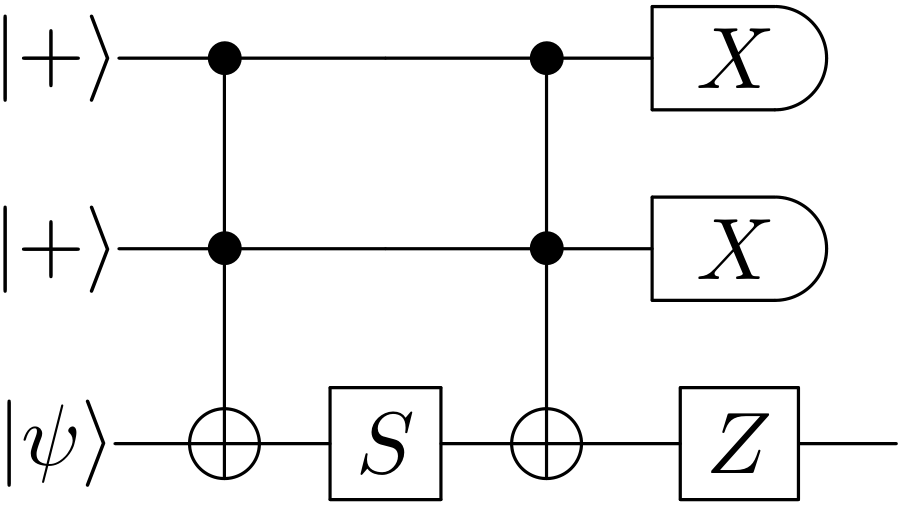
\includegraphics[width=\textwidth]{rus1.png}
    \end{minipage}
    \quad
    \begin{minipage}{0.3\textwidth}
      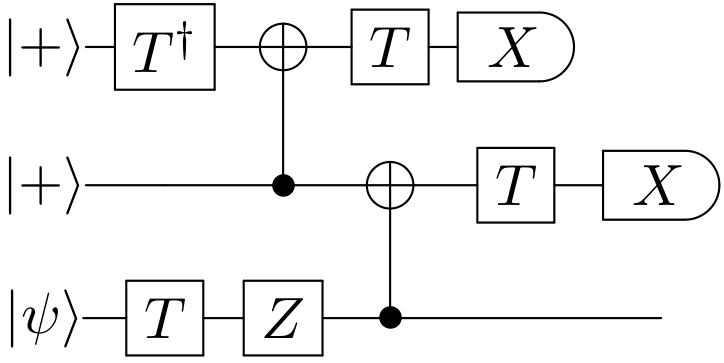
\includegraphics[width=\textwidth]{rus2.png}
    \end{minipage}
    \caption{\Large Circuit Equivalence Checking}
  \end{figure}
\end{frame}
\begin{frame}
  \begin{figure}
    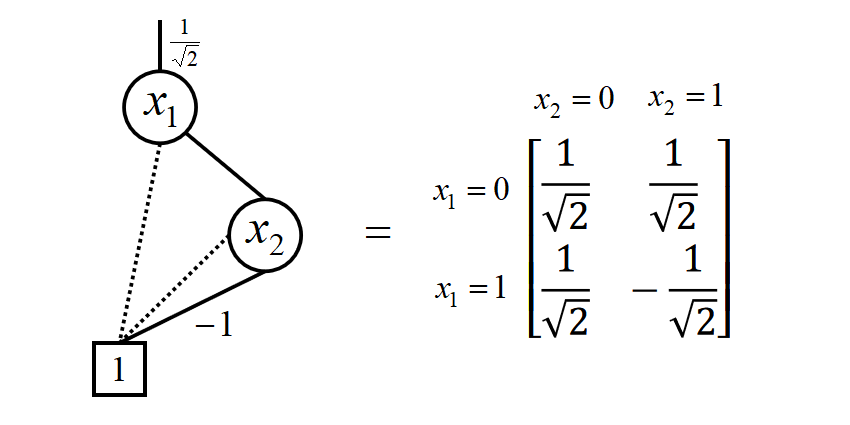
\includegraphics[width = .8\textwidth]{TDD_H_gate2.png}
    \caption{\Large a TDD example}
  \end{figure}
\end{frame}
\begin{frame}
  \begin{figure}[tbh]
      \centering
      \scalebox{0.8}{
      \begin{minipage}{0.3\textwidth}
      \small
    \[P=\frac{1}{6}\begin{bmatrix}
    1&-1  &1&-1  & 1&-1 &0&0\\
    -1&1  &-1&1  & -1&1 &0&0\\
    1&-1  &1&-1  & 1&-1 &0&0\\
    -1&1  &-1&1  & -1&1 &0&0\\
    1&-1  &1&-1  & 1&-1 &0&0\\
    -1&1  &-1&1  & -1&1 &0&0\\
    0&0   &0&0   &0&0   &3&-3\\
    0&0   &0&0   &0&0   &-3&3\\
    \end{bmatrix}
    \]
      \end{minipage}
     }
     \quad
     \hfil
      \begin{minipage}{0.5\textwidth}  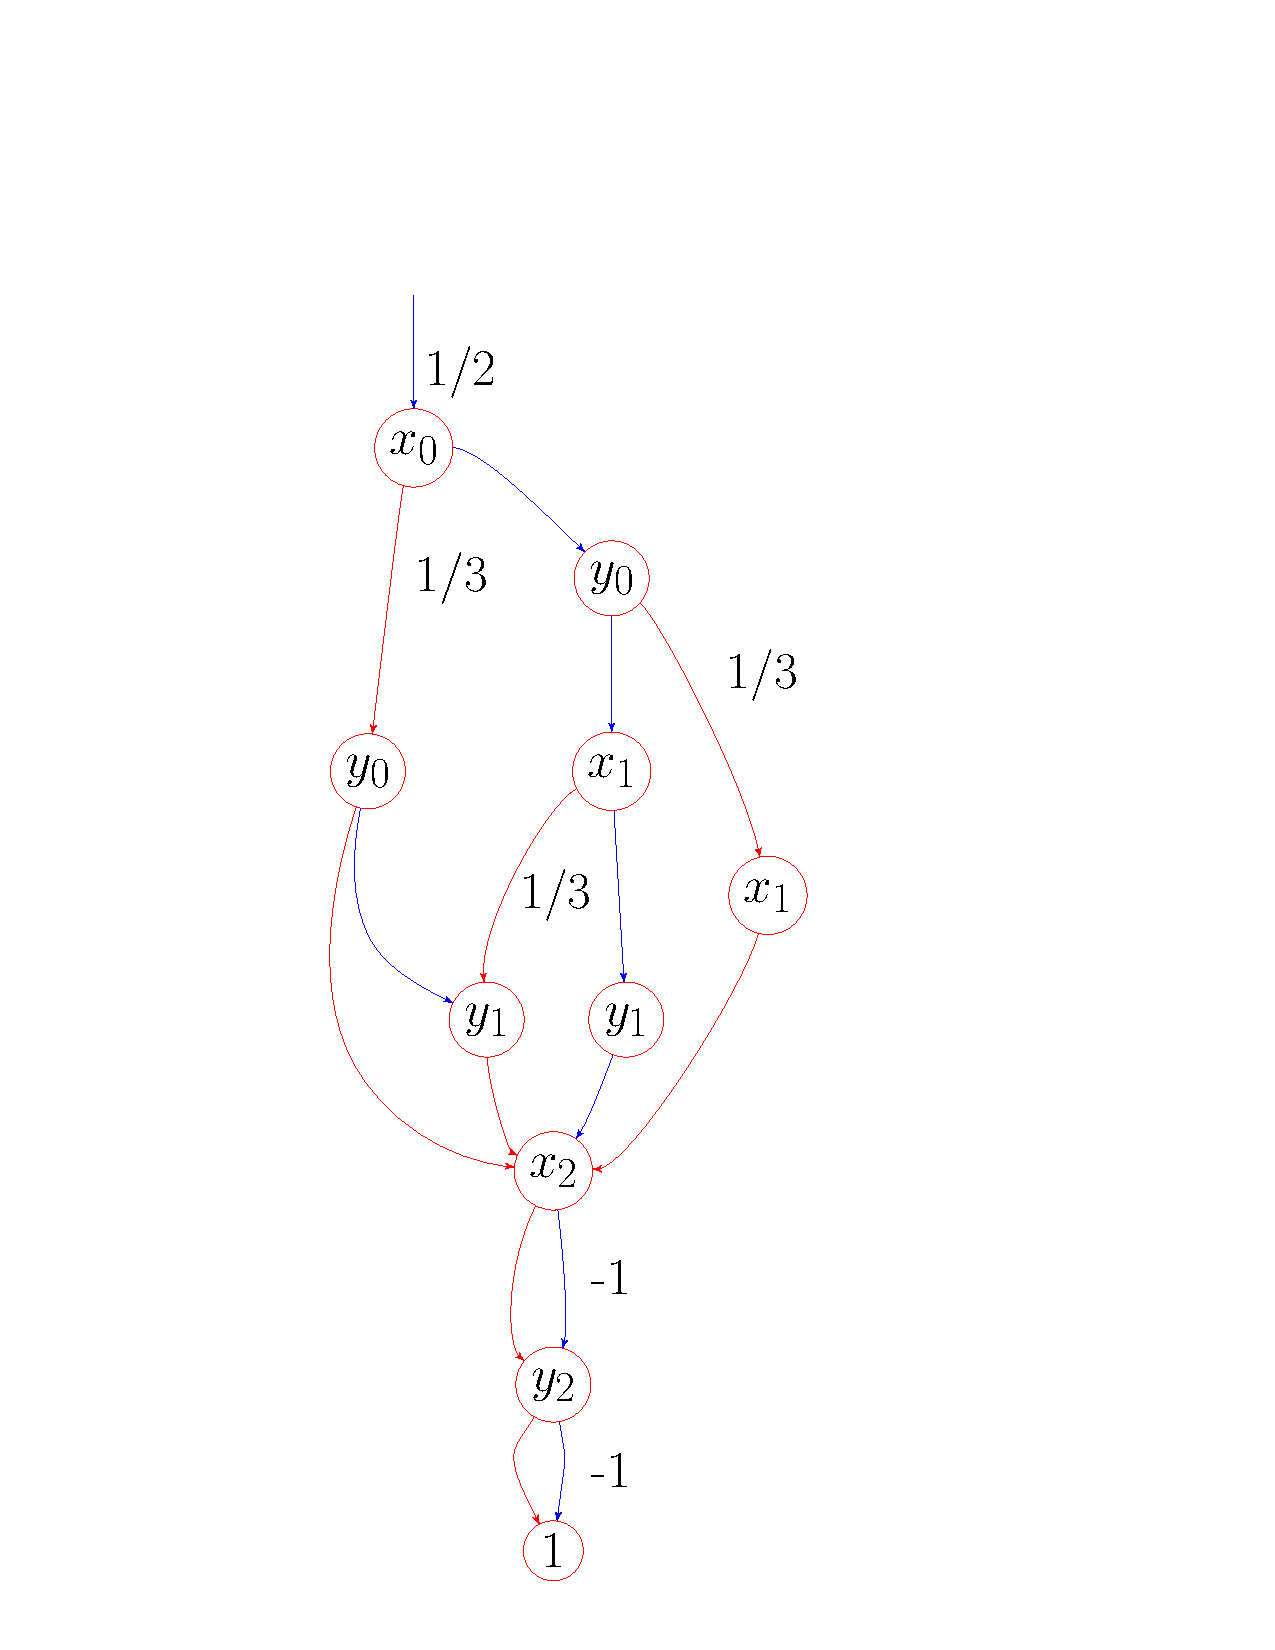
\includegraphics[width=\textwidth]{Projector.pdf}
      \end{minipage}
    \end{figure}
\end{frame}
\begin{frame}
  \begin{enumerate}
    \Large
    \item \textbf{Background and significance}
    \item \textbf{Research of related work}
    \item Future work plan
  \end{enumerate}
\end{frame}
\begin{frame}
  \begin{enumerate}
    \Large
    \item efficient quantum image computation algorithms
    \item contraction partition-based algorithm
  \end{enumerate}
\end{frame}
\end{document}